\documentclass[12pt,fleqn]{article}\usepackage{../../common}
\begin{document}
Say�sal Entegrasyon (Numerical Integration)

$F(x)$ fonksiyonunu bazen sembolik olarak entegre etmek zor olabilir. Bu
durumlarda say�sal ��z�m daha kullan��l� olabilir. Mesela $F(x)$'in $x_0$
ve $x_1$ aras�ndaki entegrali asl�nda bir alan hesab�d�r, ve bu alan�, $x$
aral���n� ufak par�alara b�lerek, ve bu par�alar� kullanarak yakla��k bir
alan hesab� yap�p sonu�lar� toplayarak elde edebiliriz. 

$x_0$ ve $x_1$ aras�n� $N$ par�aya b�lelim. 

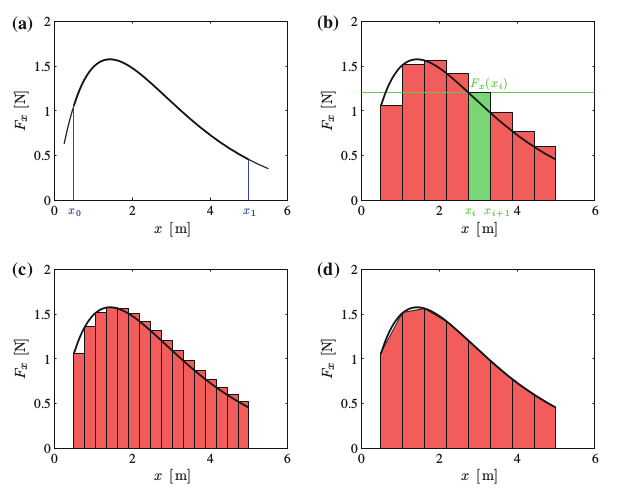
\includegraphics[width=25em]{compscieng_app01numint_01.png}






Kaynaklar

[1] Sorenssen, {\em Elementary Mechanics Using Python}

\end{document}
